% =====================================================================
% WACMR Analytics, DSM Final Project Presentation
% Build: bash build.sh
% =====================================================================
\documentclass[aspectratio=169,10pt]{beamer}

\usepackage[T1]{fontenc}
\usepackage[utf8]{inputenc}
\usepackage{lmodern}
\usepackage{microtype}
\usepackage{graphicx}
\usepackage{booktabs}
\usepackage{tabularx}
\usepackage{array}
\usepackage{amsmath}
\usepackage{amssymb}
\usepackage{tikz}
\usetikzlibrary{arrows.meta,positioning,calc,shapes.geometric}
\usepackage{ragged2e}

\graphicspath{{assets/}{../final/visualizations/}{../final/diagram/}}

% ---------------------------------------------------------------------
% Visual system
% ---------------------------------------------------------------------
\definecolor{Ink}{HTML}{17202A}
\definecolor{Slate}{HTML}{16324F}
\definecolor{Teal}{HTML}{0B7285}
\definecolor{TealTint}{HTML}{E6F4F1}
\definecolor{Amber}{HTML}{B26A00}
\definecolor{AmberTint}{HTML}{FFF4D6}
\definecolor{Rose}{HTML}{A61E4D}
\definecolor{RoseTint}{HTML}{FFF0F6}
\definecolor{Forest}{HTML}{2B6E3F}
\definecolor{ForestTint}{HTML}{E7F4EA}
\definecolor{SoftGray}{HTML}{F5F7FA}
\definecolor{LineGray}{HTML}{D8E1EA}
\definecolor{Pale}{HTML}{FBFCFE}

\setbeamersize{text margin left=0.38cm,text margin right=0.38cm}
\setbeamertemplate{navigation symbols}{}
\setbeamertemplate{headline}{}
\setbeamertemplate{frametitle}{%
  \vspace{0.13cm}
  \begin{beamercolorbox}[wd=\paperwidth,leftskip=0.38cm,rightskip=0.38cm]{frametitle}
    \usebeamerfont{frametitle}\insertframetitle
  \end{beamercolorbox}
  \vspace{-0.08cm}
  {\color{Teal}\rule{\textwidth}{0.45pt}}
  \vspace{-0.22cm}
}
\setbeamertemplate{footline}{%
  \leavevmode
  \hbox{%
    \begin{beamercolorbox}[wd=.79\paperwidth,ht=2.45ex,dp=.9ex,leftskip=1em]{author in head/foot}
      \color{Slate}\scriptsize WACMR Analytics \hspace{0.45em}| \hspace{0.45em} DSM Final Project
    \end{beamercolorbox}%
    \begin{beamercolorbox}[wd=.21\paperwidth,ht=2.45ex,dp=.9ex,rightskip=1em plus1fil]{date in head/foot}
      \color{Slate}\scriptsize \insertframenumber/\inserttotalframenumber
    \end{beamercolorbox}}%
}
\setbeamercolor{background canvas}{bg=white}
\setbeamercolor{normal text}{fg=Ink}
\setbeamercolor{frametitle}{fg=Slate}
\setbeamerfont{frametitle}{series=\bfseries,size=\Large}
\setbeamerfont{title}{series=\bfseries,size=\huge}
\setbeamerfont{subtitle}{size=\large}
\renewcommand{\arraystretch}{1.08}
\setlength{\parskip}{0.08em}

\newcolumntype{Y}{>{\RaggedRight\arraybackslash}X}
\newcommand{\tightlist}{\setlength{\itemsep}{0.10em}\setlength{\parskip}{0em}}
\newcommand{\smalltight}{\scriptsize\setlength{\itemsep}{0.08em}\setlength{\parskip}{0em}}
\newcommand{\kpi}[4][Slate]{%
  \begin{tikzpicture}
    \node[draw=#1!70,fill=#1!8,rounded corners=2pt,inner sep=4.6pt,
      minimum height=1.03cm,text width=\dimexpr\linewidth-10pt\relax,align=left] {
      {\color{#1}\bfseries\large #2}\\[-2pt]
      {\scriptsize #3}\\[-1pt]
      {\tiny\color{Ink!68}#4}
    };
  \end{tikzpicture}%
}
\newcommand{\card}[3]{%
  \begin{tikzpicture}
    \node[draw=#1!70,fill=#1!8,rounded corners=2pt,inner sep=4.8pt,
      text width=\dimexpr\linewidth-11pt\relax,align=left] {
      {\color{#1}\bfseries #2}\\[-1pt]{\scriptsize #3}
    };
  \end{tikzpicture}%
}
\newcommand{\callout}[2][Teal]{%
  \begin{tikzpicture}
    \node[draw=#1!70,fill=#1!9,rounded corners=2pt,inner sep=5pt,
      text width=\dimexpr\linewidth-12pt\relax,align=left] {\small #2};
  \end{tikzpicture}%
}
\newcommand{\pill}[2]{%
  \tikz[baseline=(n.base)]\node[draw=#1!75,fill=#1!10,rounded corners=2pt,
    inner xsep=4pt,inner ysep=1.6pt](n){\tiny\bfseries #2};%
}
\newcommand{\formulaNote}[1]{{\scriptsize\color{Ink!72}#1}}
\newcommand{\figband}[3]{%
  \begin{center}
    \includegraphics[width=#1,height=#2,keepaspectratio]{#3}
  \end{center}
}

\title{Predicting India's Weighted Average Call Money Rate}
\author{Aamer Jalan and Arnav Goyal}
\institute{Ashoka University, Data Science and Management}
\date{April 26, 2026}

\begin{document}

% ---------------------------------------------------------------------
% SLIDE 1
% ---------------------------------------------------------------------
\begin{frame}[plain]
  \begin{tikzpicture}[remember picture,overlay]
    \fill[Slate] (current page.north west) rectangle ([yshift=-1.02cm]current page.north east);
    \fill[Teal] ([yshift=-1.02cm]current page.north west) rectangle ([yshift=-1.10cm]current page.north east);
  \end{tikzpicture}
  \vspace{0.18cm}
  {\color{white}\bfseries Ashoka University, Data Science and Management}\par
  \vspace{0.65cm}
  \begin{center}
    {\usebeamerfont{title}\color{Slate}\inserttitle\par}
    \vspace{0.22cm}
    {\usebeamerfont{subtitle}\color{Teal}\insertsubtitle\par}
    \vspace{0.45cm}
    {\large \insertauthor} \\
    \vspace{0.10cm}
    {\small \insertdate}
  \end{center}
  \vfill
  \begin{columns}[T,totalwidth=\linewidth]
    \column{0.19\linewidth}\kpi{545}{weeks}{}
    \column{0.19\linewidth}\kpi[Teal]{117}{features}{}
    \column{0.19\linewidth}\kpi[Amber]{10}{data sources}{}
    \column{0.19\linewidth}\kpi[Forest]{70.9\%}{directional accuracy}{}
    \column{0.19\linewidth}\kpi[Rose]{75}{policy events}{}
  \end{columns}
\end{frame}

% ---------------------------------------------------------------------
% SLIDE 2
% ---------------------------------------------------------------------
\begin{frame}{What is WACMR? (The Problem)}
  \begin{columns}[T,totalwidth=\textwidth]
    \column{0.48\textwidth}
      {\color{Slate}\bfseries What is WACMR?}\par
      \vspace{0.2cm}
      \begin{itemize}\small
        \item Overnight interbank lending rate for scheduled commercial banks.
        \item Volume-weighted rate across all transactions in a given day/week.
        \item The operational target of the RBI's Liquidity Adjustment Facility (LAF).
      \end{itemize}
    \column{0.48\textwidth}
      {\color{Slate}\bfseries Why does it matter?}\par
      \vspace{0.2cm}
      \begin{itemize}\small
        \item \textbf{RBI:} Policy enforcement \& monitoring liquidity.
        \item \textbf{Banks \& Funds:} Treasury and overnight fund NAV decisions.
        \item \textbf{Researchers:} Regime analysis \& monetary transmission.
      \end{itemize}
  \end{columns}
  \vfill
  \callout[Amber]{\textbf{Key Fact:} WACMR moves first when liquidity tightens or loosens — before the rest of the rate curve follows.}
\end{frame}

% ---------------------------------------------------------------------
% SLIDE 3
% ---------------------------------------------------------------------
\begin{frame}{The Five Channels (Why It's Hard to Predict)}
  \begin{center}
    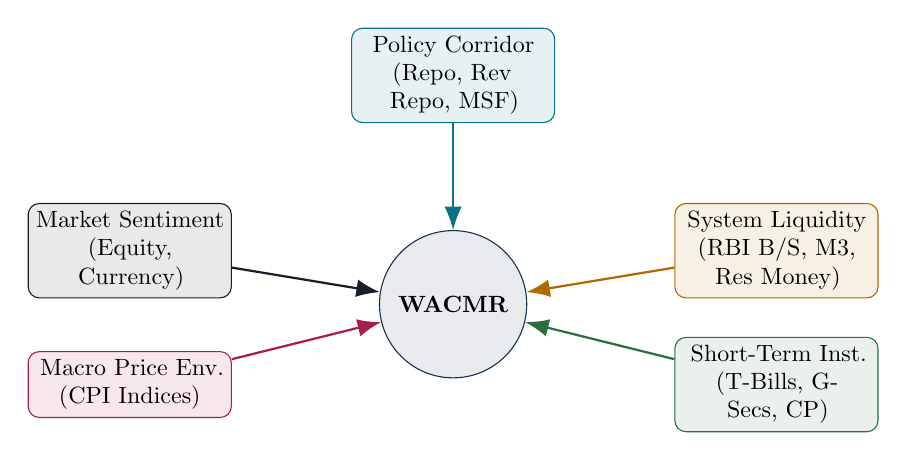
\begin{tikzpicture}[scale=0.85, transform shape, node distance=2.5cm, every node/.style={align=center}]
      \node[draw=Slate, fill=Slate!10, circle, minimum size=2.2cm, font=\bfseries] (center) {WACMR};
      
      \node[draw=Teal, fill=Teal!10, rounded corners, text width=2.8cm, above=1.6cm of center] (n1) {Policy Corridor\\(Repo, Rev Repo, MSF)};
      \node[draw=Amber, fill=Amber!10, rounded corners, text width=2.8cm, right=2.2cm of center, yshift=0.8cm] (n2) {System Liquidity\\(RBI B/S, M3, Res Money)};
      \node[draw=Forest, fill=Forest!10, rounded corners, text width=2.8cm, right=2.2cm of center, yshift=-1.2cm] (n3) {Short-Term Inst.\\(T-Bills, G-Secs, CP)};
      \node[draw=Rose, fill=Rose!10, rounded corners, text width=2.8cm, left=2.2cm of center, yshift=-1.2cm] (n4) {Macro Price Env.\\(CPI Indices)};
      \node[draw=Ink, fill=Ink!10, rounded corners, text width=2.8cm, left=2.2cm of center, yshift=0.8cm] (n5) {Market Sentiment\\(Equity, Currency)};
      
      \draw[-{Latex[length=3mm]}, thick, Teal] (n1) -- (center);
      \draw[-{Latex[length=3mm]}, thick, Amber] (n2) -- (center);
      \draw[-{Latex[length=3mm]}, thick, Forest] (n3) -- (center);
      \draw[-{Latex[length=3mm]}, thick, Rose] (n4) -- (center);
      \draw[-{Latex[length=3mm]}, thick, Ink] (n5) -- (center);
    \end{tikzpicture}
  \end{center}
  \vfill
  \callout[Slate]{Relative weights of these channels change across structural regimes $\rightarrow$ non-stationary problem.}
\end{frame}

% ---------------------------------------------------------------------
% SLIDE 4
% ---------------------------------------------------------------------
\begin{frame}{Our Four Hypotheses}
  \begin{columns}[T,totalwidth=\textwidth]
    \column{0.48\textwidth}
      \card{Slate}{H1: Regime Structure}{India's money market data contains at least 2 statistically distinct macroeconomic regimes.\hfill\textbf{?}}
      \vspace{0.4cm}
      \card{Teal}{H2: Regime-Aware Forecasting}{Injecting regime labels reduces out-of-sample RMSE by $\geq$15\%.\hfill\textbf{?}}
    \column{0.48\textwidth}
      \card{Amber}{H3: Corridor Dominance}{Repo, Reverse Repo, MSF are the top SHAP predictors.\hfill\textbf{?}}
      \vspace{0.4cm}
      \card{Forest}{H4: Market Sentiment}{Adding 28 Nifty/USD-INR features materially improves forecasting.\hfill\textbf{?}}
  \end{columns}
\end{frame}

% ---------------------------------------------------------------------
% SLIDE 5
% ---------------------------------------------------------------------
\begin{frame}{Data Sources Overview}
  \begin{columns}[T,totalwidth=\textwidth]
    \column{0.32\textwidth}
      \card{Slate}{NDAP API — 8 RBI Datasets}{}
      {\scriptsize
      \begin{tabularx}{\linewidth}{@{}p{0.45\linewidth}Y@{}}
        \toprule
        \textbf{Domain} & \textbf{Dataset Name} \\
        \midrule
        Monetary Policy & RBI Ratios \& Rates \\
        Central Bank B/S & Liabilities \& Assets \\
        Money Supply & Weekly Aggregates \\
        Debt Markets & CP Details \\
        Debt Markets & T-Bills Details \\
        Repo Markets & Market Repo Trans. \\
        Debt Markets & Govt Dated Secs \\
        Inflation & Major Price Indices \\
        \bottomrule
      \end{tabularx}}
    \column{0.32\textwidth}
      \card{Teal}{Yahoo Finance — 2 Datasets}{}
      \vspace{0.1cm}
      \begin{itemize}\scriptsize
        \item Nifty 50 (\textasciicircum NSEI) Weekly OHLCV
        \item USD/INR (USDINR=X) Weekly OHLCV
      \end{itemize}
    \column{0.32\textwidth}
      \card{Amber}{Curated NLP Corpus}{}
      \vspace{0.1cm}
      \begin{itemize}\scriptsize
        \item 75 RBI policy events
        \item Feb 2014 – Aug 2024
        \item 6 categories
        \item Sentiment scores [$-1, +1$]
      \end{itemize}
  \end{columns}
  \vfill
  \callout[Forest]{\textbf{February 2014 $\rightarrow$ July 2024} | 545 Friday-aligned weekly observations | 119 columns}
\end{frame}

% ---------------------------------------------------------------------
% SLIDE 6
% ---------------------------------------------------------------------
\begin{frame}{Data Engineering: The Friday-Alignment Problem}
  \begin{center}
    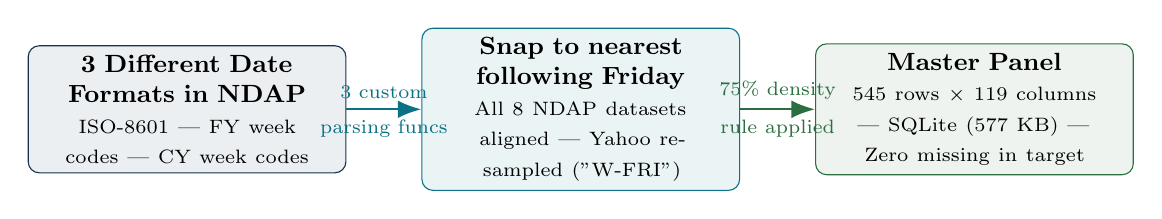
\begin{tikzpicture}[x=1cm,y=1cm,every node/.style={font=\small, align=center}]
      \node[draw=Slate,fill=Slate!8,rounded corners,text width=3.8cm,minimum height=1.5cm] (step1) at (0,0) {
        \textbf{3 Different Date}\\
        \textbf{Formats in NDAP}\\
        \scriptsize ISO-8601 | FY week codes | CY week codes
      };
      
      \node[draw=Teal,fill=Teal!8,rounded corners,text width=3.8cm,minimum height=1.5cm] (step2) at (5,0) {
        \textbf{Snap to nearest}\\
        \textbf{following Friday}\\
        \scriptsize All 8 NDAP datasets aligned | Yahoo resampled ("W-FRI")
      };
      
      \node[draw=Forest,fill=Forest!8,rounded corners,text width=3.8cm,minimum height=1.5cm] (step3) at (10,0) {
        \textbf{Master Panel}\\
        \scriptsize 545 rows $\times$ 119 columns | SQLite (577 KB) | Zero missing in target
      };
      
      \draw[-{Latex[length=3mm]},thick,Teal] (step1) -- node[above]{\scriptsize 3 custom} node[below]{\scriptsize parsing funcs} (step2);
      \draw[-{Latex[length=3mm]},thick,Forest] (step2) -- node[above]{\scriptsize 75\% density} node[below]{\scriptsize rule applied} (step3);
    \end{tikzpicture}
  \end{center}
  \vfill
  \callout[Rose]{Without custom parsing, dates off by up to 12 weeks for financial-year tables.}
\end{frame}

% ---------------------------------------------------------------------
% SLIDE 7
% ---------------------------------------------------------------------
\begin{frame}{Exploratory Data Analysis: WACMR Over Time}
  \figband{\linewidth}{4.2cm}{target_timeseries.png}
  \vspace{-0.2cm}
  {\scriptsize Annotations: "Post-taper tantrum peak (8.90\%)" | "Demonetisation spike $\downarrow$ Nov 2016" | "COVID crash $\downarrow$ Mar 2020" | "Re-tightening begins mid-2022"}
  \vspace{0.2cm}
  \begin{columns}[T,totalwidth=\linewidth]
    \column{0.24\linewidth}\kpi{5.803\%}{Mean}{}
    \column{0.24\linewidth}\kpi[Teal]{1.462\%}{Std Dev}{}
    \column{0.24\linewidth}\kpi[Amber]{3.07\%}{Min}{(Dec 2020)}
    \column{0.24\linewidth}\kpi[Rose]{8.90\%}{Max}{(Feb 2014)}
  \end{columns}
  \vfill
  \callout[Slate]{Visually bimodal — two distinct eras visible to the naked eye.}
\end{frame}

% ---------------------------------------------------------------------
% SLIDE 8
% ---------------------------------------------------------------------
\begin{frame}{EDA: Bimodal Distribution and Correlation Findings}
  \begin{columns}[T,totalwidth=\textwidth]
    \column{0.48\textwidth}
      {\color{Slate}\bfseries Bimodal Density}\\
      {\scriptsize Peak 1: "Surplus Liquidity $\sim$3.3\%" | Peak 2: "Tight Liquidity $\sim$6.5\%"}\par
      \vspace{0.1cm}
      \figband{\linewidth}{3.5cm}{eda_distributions.png}
      \vspace{0.1cm}
      \callout[Teal]{Bimodality signals regime non-stationarity.}
    \column{0.48\textwidth}
      {\color{Slate}\bfseries Top Non-Corridor Correlations}\par
      \vspace{0.1cm}
      {\scriptsize
      \begin{tabularx}{\linewidth}{@{}p{0.35\linewidth}Yc@{}}
        \toprule
        \textbf{Feature} & \textbf{Domain} & \textbf{Pearson r} \\
        \midrule
        CBLO Rate & Debt & 0.96 \\
        CD Rate & Debt & 0.85 \\
        CP Outstanding & Commercial Paper & 0.42 \\
        USD/INR & Forex & $-$0.18 \\
        Nifty 50 & Equity & $-$0.27 \\
        \bottomrule
      \end{tabularx}}
      \vspace{0.3cm}
      \callout[Amber]{Equity and forex already look weak here.}
  \end{columns}
\end{frame}

% ---------------------------------------------------------------------
% SLIDE 9
% ---------------------------------------------------------------------
\begin{frame}{Project Pipeline at a Glance}
  \begin{center}
    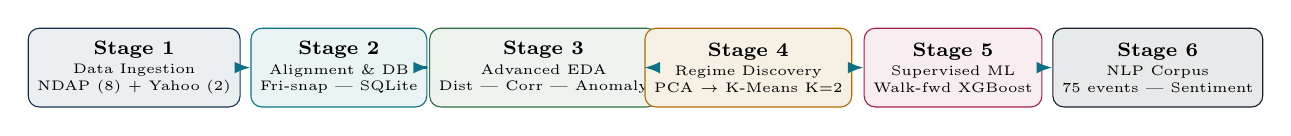
\begin{tikzpicture}[x=1cm,y=1cm,every node/.style={font=\scriptsize, align=center}]
      \node[draw=Slate,fill=Slate!8,rounded corners,minimum width=2.2cm,minimum height=1.0cm] (s1) at (0,0) {
        \textbf{Stage 1}\\[-1pt] \tiny Data Ingestion\\[-2pt] \tiny NDAP (8) + Yahoo (2)
      };
      \node[draw=Teal,fill=Teal!8,rounded corners,minimum width=2.2cm,minimum height=1.0cm] (s2) at (2.6,0) {
        \textbf{Stage 2}\\[-1pt] \tiny Alignment \& DB\\[-2pt] \tiny Fri-snap | SQLite
      };
      \node[draw=Forest,fill=Forest!8,rounded corners,minimum width=2.2cm,minimum height=1.0cm] (s3) at (5.2,0) {
        \textbf{Stage 3}\\[-1pt] \tiny Advanced EDA\\[-2pt] \tiny Dist | Corr | Anomaly
      };
      \node[draw=Amber,fill=Amber!10,rounded corners,minimum width=2.2cm,minimum height=1.0cm] (s4) at (7.8,0) {
        \textbf{Stage 4}\\[-1pt] \tiny Regime Discovery\\[-2pt] \tiny PCA $\rightarrow$ K-Means K=2
      };
      \node[draw=Rose,fill=Rose!8,rounded corners,minimum width=2.2cm,minimum height=1.0cm] (s5) at (10.4,0) {
        \textbf{Stage 5}\\[-1pt] \tiny Supervised ML\\[-2pt] \tiny Walk-fwd XGBoost
      };
      \node[draw=Ink,fill=Ink!10,rounded corners,minimum width=2.2cm,minimum height=1.0cm] (s6) at (13.0,0) {
        \textbf{Stage 6}\\[-1pt] \tiny NLP Corpus\\[-2pt] \tiny 75 events | Sentiment
      };
      
      \foreach \x/\y in {s1/s2,s2/s3,s3/s4,s4/s5,s5/s6}
        \draw[-{Latex[length=2mm]},thick,Teal] (\x) -- (\y);
    \end{tikzpicture}
  \end{center}
  \vspace{0.1cm}
  \callout[Slate]{Each stage is idempotent and reads only from the previous stage's persisted output.}
\end{frame}

% ---------------------------------------------------------------------
% SLIDE 10
% ---------------------------------------------------------------------
\begin{frame}{Regime Discovery: PCA + K-Means}
  \begin{columns}[T,totalwidth=\textwidth]
    \column{0.48\textwidth}
      {\color{Slate}\bfseries How We Did It}\par
      \vspace{0.2cm}
      \begin{itemize}
        \item \textbf{Step 1}: StandardScaler (zero mean, unit variance)
        \item \textbf{Step 2}: PCA $\rightarrow$ 14 components retain 90.4\% variance
        \item \textbf{Step 3}: K-Means sweep K=2 to K=7
        \item \textbf{Metric}: Silhouette score
      \end{itemize}
    \column{0.48\textwidth}
      {\color{Slate}\bfseries Silhouette Sweep Results}\par
      \vspace{0.2cm}
      {\small
      \begin{tabularx}{\linewidth}{@{}p{0.25\linewidth}Y@{}}
        \toprule
        \textbf{K} & \textbf{Silhouette Score} \\
        \midrule
        K=2 & 0.4238 \textbf{\checkmark OPTIMAL} \\
        K=3 & 0.4048 \\
        K=4 & 0.3321 \\
        K=5 & 0.3351 \\
        K=6 & 0.3205 \\
        K=7 & 0.3022 \\
        \bottomrule
      \end{tabularx}}
  \end{columns}
  \vfill
  \callout[Teal]{K=2 wins on both silhouette score AND macroeconomic interpretability.}
\end{frame}

% ---------------------------------------------------------------------
% SLIDE 11
% ---------------------------------------------------------------------
\begin{frame}{The Two Discovered Regimes}
  \begin{columns}[T,totalwidth=\textwidth]
    \column{0.48\textwidth}
      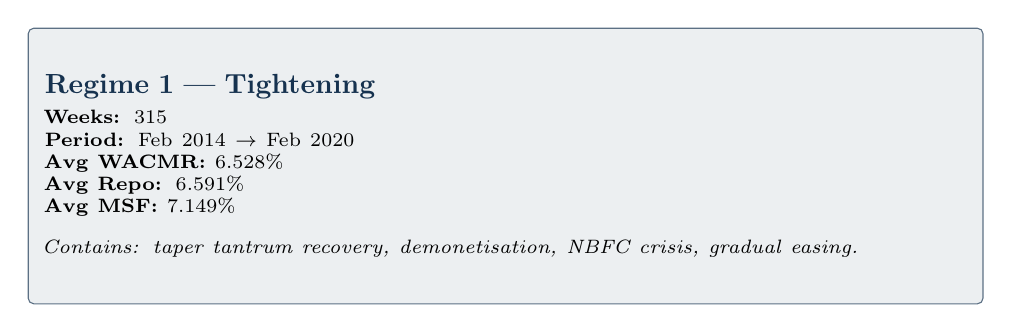
\begin{tikzpicture}
        \node[draw=Slate!70,fill=Slate!8,rounded corners=2pt,inner sep=6pt,
          text width=\dimexpr\linewidth-12pt\relax,align=left,minimum height=3.5cm] {
          {\color{Slate}\bfseries Regime 1 — Tightening}\\[0.1cm]
          \scriptsize \textbf{Weeks:} 315\\
          \scriptsize \textbf{Period:} Feb 2014 $\rightarrow$ Feb 2020\\
          \scriptsize \textbf{Avg WACMR:} 6.528\%\\
          \scriptsize \textbf{Avg Repo:} 6.591\%\\
          \scriptsize \textbf{Avg MSF:} 7.149\%\\[0.1cm]
          \scriptsize \textit{Contains: taper tantrum recovery, demonetisation, NBFC crisis, gradual easing.}
        };
      \end{tikzpicture}
    \column{0.48\textwidth}
      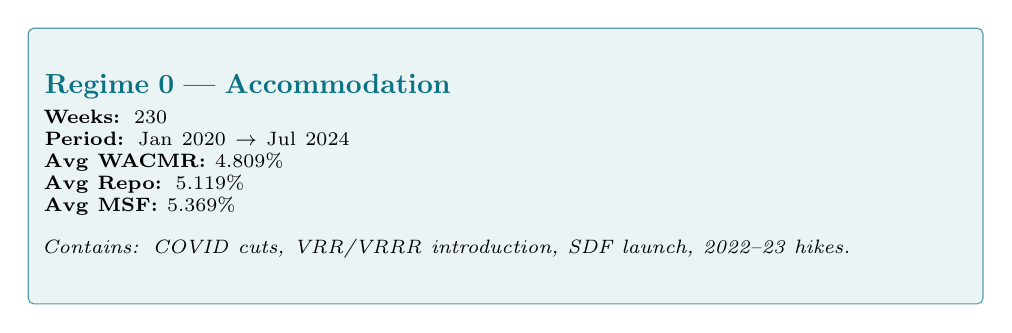
\begin{tikzpicture}
        \node[draw=Teal!70,fill=Teal!8,rounded corners=2pt,inner sep=6pt,
          text width=\dimexpr\linewidth-12pt\relax,align=left,minimum height=3.5cm] {
          {\color{Teal}\bfseries Regime 0 — Accommodation}\\[0.1cm]
          \scriptsize \textbf{Weeks:} 230\\
          \scriptsize \textbf{Period:} Jan 2020 $\rightarrow$ Jul 2024\\
          \scriptsize \textbf{Avg WACMR:} 4.809\%\\
          \scriptsize \textbf{Avg Repo:} 5.119\%\\
          \scriptsize \textbf{Avg MSF:} 5.369\%\\[0.1cm]
          \scriptsize \textit{Contains: COVID cuts, VRR/VRRR introduction, SDF launch, 2022–23 hikes.}
        };
      \end{tikzpicture}
  \end{columns}
  \vfill
  \callout[Amber]{Gap between regime means: 1.72 percentage points — real, not a statistical artefact.}
  \vspace{0.1cm}
  \callout[Forest]{\textbf{Key insight:} Even the 2022–23 hiking cycle stays classified as Regime 0 — the operational framework changed permanently.}
\end{frame}

% ---------------------------------------------------------------------
% SLIDE 12
% ---------------------------------------------------------------------
\begin{frame}{PCA Scatter + Regime Timeline}
  \begin{columns}[T,totalwidth=\textwidth]
    \column{0.48\textwidth}
      \figband{\linewidth}{3.5cm}{pca_regime_scatter.png}
      \vspace{0.1cm}
      {\scriptsize \textit{Two clusters well-separated along PC1 (49.9\% variance)}}
    \column{0.48\textwidth}
      \figband{\linewidth}{3.5cm}{regime_timeseries.png}
      \vspace{0.1cm}
      {\scriptsize \textit{Clean break in early 2020 — visible as both a colour change and a level shift}}
  \end{columns}
  \vfill
  \callout[Forest]{\textbf{\checkmark H1 CONFIRMED — Data alone identifies two statistically distinct regimes.}}
\end{frame}

% ---------------------------------------------------------------------
% SLIDE 13
% ---------------------------------------------------------------------
\begin{frame}{Supervised Forecasting: Walk-Forward Setup}
  \begin{center}
    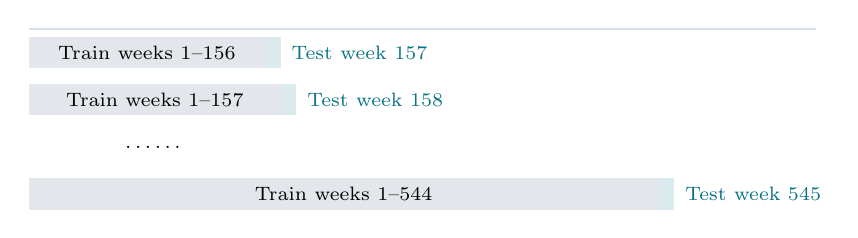
\begin{tikzpicture}[x=1cm,y=1cm,every node/.style={font=\scriptsize}]
      \draw[LineGray,thick] (0,1.5) -- (10,1.5);
      \fill[Slate!12] (0,1.0) rectangle (3.0,1.4);
      \fill[Teal!15] (3.0,1.0) rectangle (3.2,1.4);
      \node at (1.5,1.2) {Train weeks 1--156};
      \node[Teal] at (4.2,1.2) {Test week 157};
      
      \fill[Slate!12] (0,0.4) rectangle (3.2,0.8);
      \fill[Teal!15] (3.2,0.4) rectangle (3.4,0.8);
      \node at (1.6,0.6) {Train weeks 1--157};
      \node[Teal] at (4.4,0.6) {Test week 158};
      
      \node at (1.6,0.0) {\dots \dots};
      
      \fill[Slate!12] (0,-0.8) rectangle (8.0,-0.4);
      \fill[Teal!15] (8.0,-0.8) rectangle (8.2,-0.4);
      \node at (4.0,-0.6) {Train weeks 1--544};
      \node[Teal] at (9.2,-0.6) {Test week 545};
    \end{tikzpicture}
    \vspace{0.2cm}\\
    {\small \textbf{Total: 389 out-of-sample predictions}}
  \end{center}
  \vspace{0.2cm}
  \begin{columns}[T,totalwidth=\textwidth]
    \column{0.48\textwidth}
      \card{Slate}{Baseline}{117 features (corridor + balance sheet + debt + CPI + market + 3 AR lags)}
    \column{0.48\textwidth}
      \card{Teal}{Regime-Aware}{122 features (baseline + 2 one-hot regime indicators + 2 centroid distances)}
  \end{columns}
  \vfill
  \callout[Amber]{\textbf{XGBoost hyperparameters:} n\_estimators: 400 | learning\_rate: 0.05 | max\_depth: 4 | subsample: 0.8 | colsample\_bytree: 0.8 | reg\_alpha: 0.1 | reg\_lambda: 1.0}
\end{frame}

% ---------------------------------------------------------------------
% SLIDE 14
% ---------------------------------------------------------------------
\begin{frame}{Forecasting Results}
  \begin{columns}[T,totalwidth=\linewidth]
    \column{0.32\linewidth}\kpi{0.1019}{RMSE}{($\sim$10 basis points)}
    \column{0.32\linewidth}\kpi[Teal]{0.0646}{MAE}{}
    \column{0.32\linewidth}\kpi[Forest]{70.9\%}{Directional Accuracy}{}
  \end{columns}
  \vspace{0.1cm}
  \figband{\linewidth}{2.1cm}{actual_vs_predicted.png}
  \vspace{-0.1cm}
  {\scriptsize Annotations: "COVID cut Apr 2020 ($-$0.66\%)" | "Surprise hike May 2022 ($-$0.42\%)" | "Post-hike shocks 2022"}
  \vspace{0.1cm}
  {\scriptsize
  \begin{tabularx}{\linewidth}{@{}Yccc@{}}
    \toprule
    \textbf{Metric} & \textbf{Baseline} & \textbf{Regime-Aware} & \textbf{Change} \\
    \midrule
    RMSE & 0.1019 & 0.1044 & +2.5\% worse \\
    MAE & 0.0646 & 0.0646 & 0.0\% \\
    Directional Accuracy & 70.9\% & 70.9\% & +0.0pp \\
    \bottomrule
  \end{tabularx}}
  \vspace{0.1cm}
  \callout[Rose]{\textbf{$\times$ H2 REJECTED — Regime labels add no value; baseline already learns regime implicitly.}}
\end{frame}

% ---------------------------------------------------------------------
% SLIDE 15
% ---------------------------------------------------------------------
\begin{frame}{SHAP Feature Importance}
  \begin{columns}[T,totalwidth=\textwidth]
    \column{0.48\textwidth}
      \figband{\linewidth}{4.0cm}{shap_summary.png}
    \column{0.48\textwidth}
      {\color{Slate}\bfseries What SHAP Tells Us}\par
      \vspace{0.2cm}
      \begin{itemize}
        \item \textbf{Top 3 features} combined SHAP = 0.895 out of total 1.285 for top 15.
        \item \textbf{Feature groups in top 15:} corridor rates, autoregressive lags, one engineered spread, one balance sheet item.
        \item \textbf{Equity/forex features:} ZERO appearances in top 15.
        \item \textbf{First market feature:} rank 23, SHAP = 0.0038.
      \end{itemize}
      \vspace{0.1cm}
      \callout[Forest]{\textbf{\checkmark H3 CONFIRMED — Corridor rates dominate.}}
      \vspace{0.2cm}
      \callout[Rose]{\textbf{$\times$ H4 REJECTED — Equity and forex are irrelevant.}}
  \end{columns}
\end{frame}

% ---------------------------------------------------------------------
% SLIDE 16
% ---------------------------------------------------------------------
\begin{frame}{Regime-Conditional SHAP}
  \begin{columns}[T,totalwidth=\textwidth]
    \column{0.48\textwidth}
      {\color{Slate}\bfseries Regime 1 — Tightening (315 weeks)}\par
      {\scriptsize Top 12 SHAP values, target\_lag1 dominant at 0.689}
    \column{0.48\textwidth}
      {\color{Teal}\bfseries Regime 0 — Accommodation (230 weeks)}\par
      {\scriptsize Top 12 SHAP values, target\_lag1 at 0.344, Reverse Repo rises in ranking}
  \end{columns}
  \vspace{0.1cm}
  \figband{0.9\linewidth}{2.4cm}{shap_by_regime.png}
  \vspace{0.1cm}
  \callout[Amber]{\textbf{Finding 1:} Reverse Repo rises in importance in accommodation — binding constraint shifts to lower corridor floor.}
  \vspace{0.1cm}
  \callout[Forest]{\textbf{Finding 2:} All SHAP magnitudes $\sim$2$\times$ larger in tightening — WACMR is more predictable when RBI is tightening.}
\end{frame}

% ---------------------------------------------------------------------
% SLIDE 17
% ---------------------------------------------------------------------
\begin{frame}{Residual Analysis: What the Model Gets Wrong}
  \figband{0.9\linewidth}{3.5cm}{residual_calendar.png}
  \vspace{0.2cm}
  \begin{columns}[T,totalwidth=\textwidth]
    \column{0.48\textwidth}
      \card{Slate}{Calendar Events — NOT the problem}{
        \begin{itemize}
          \item 66 calendar-event weeks tested
          \item RMSE on calendar weeks: 0.0870
          \item RMSE on non-calendar weeks: 0.1046
          \item \textit{Model handles seasonal patterns — 10 years of training is enough.}
        \end{itemize}
      }
    \column{0.48\textwidth}
      \card{Rose}{Policy Surprises — THE real problem}{
        \begin{itemize}
          \item COVID cut Apr 2020: $-$0.66\% miss
          \item Surprise hike May 2022: $-$0.42\% miss
          \item Post-hike shocks 2022: 0.30–0.34\% miss
          \item \textit{By definition unforecastable from historical features.}
        \end{itemize}
      }
  \end{columns}
\end{frame}

% ---------------------------------------------------------------------
% SLIDE 18
% ---------------------------------------------------------------------
\begin{frame}{NLP Corpus and Event Analysis}
  \begin{columns}[T,totalwidth=\textwidth]
    \column{0.19\linewidth}\kpi{75}{events}{}
    \column{0.19\linewidth}\kpi[Teal]{6}{categories}{}
    \column{0.19\linewidth}\kpi[Amber]{10}{years (Feb 14-Aug 24)}{}
    \column{0.19\linewidth}\kpi[Forest]{[$-$1, +1]}{sentiment}{}
    \column{0.19\linewidth}\kpi[Rose]{RBI/News}{sources}{}
  \end{columns}
  \vspace{0.2cm}
  \begin{columns}[T,totalwidth=\textwidth]
    \column{0.48\textwidth}
      \figband{\linewidth}{3cm}{news_sentiment_timeline.png}
    \column{0.48\textwidth}
      \figband{\linewidth}{3cm}{event_density_heatmap.png}
  \end{columns}
  \vspace{0.2cm}
  \callout[Slate]{Pearson r = $-$0.21 between weekly sentiment and WACMR change — dovish weeks associated with falling WACMR | Signal too weak to use as primary feature but validates qualitative event overlay.}
  \vspace{0.1cm}
  {\scriptsize \textit{Why manual curation? Off-the-shelf models (VADER, FinBERT) misclassify Indian monetary policy language.}}
\end{frame}

% ---------------------------------------------------------------------
% SLIDE 19
% ---------------------------------------------------------------------
\begin{frame}{Hypothesis Verdicts Summary}
  {\color{Slate}\bfseries All Four Hypotheses — Final Verdicts}\par
  \vspace{0.2cm}
  {\small
  \begin{tabularx}{\linewidth}{@{}p{0.22\linewidth}p{0.18\linewidth}cp{0.36\linewidth}@{}}
    \toprule
    \textbf{Hypothesis} & \textbf{Prediction} & \textbf{Verdict} & \textbf{Key Evidence} \\
    \midrule
    \textbf{H1} — Regime structure exists & $\geq$2 distinct regimes & {\color{Forest}\bfseries \checkmark CONFIRMED} & K-Means K=2, silhouette 0.4238, aligns with COVID break \\
    \midrule
    \textbf{H2} — Regime labels improve forecasts & $\geq$15\% RMSE reduction & {\color{Rose}\bfseries $\times$ REJECTED} & Regime-aware RMSE 0.1044 vs baseline 0.1019 (+2.5\% worse) \\
    \midrule
    \textbf{H3} — Corridor rates dominate & Top SHAP features & {\color{Forest}\bfseries \checkmark CONFIRMED} & Repo, Reverse Repo, MSF + AR lags fill entire top 15 \\
    \midrule
    \textbf{H4} — Equity/forex add value & Meaningful RMSE improvement & {\color{Rose}\bfseries $\times$ REJECTED} & First market feature at rank 23, SHAP 100$\times$ smaller than corridor \\
    \bottomrule
  \end{tabularx}}
\end{frame}

% ---------------------------------------------------------------------
% SLIDE 20
% ---------------------------------------------------------------------
\begin{frame}{What the Data Says: Five Economic Claims}
  \vspace{0.1cm}
  \card{Slate}{1. The 2020 break is structural, not transitional}{Even 2022–23 hikes operate inside the new framework.}
  \vspace{0.15cm}
  \card{Teal}{2. The policy corridor explains almost everything}{Equity and forex explain almost nothing.}
  \vspace{0.15cm}
  \card{Forest}{3. Forecasting to $\sim$10 basis points is feasible}{Explicit regime tagging adds no value.}
  \vspace{0.15cm}
  \card{Rose}{4. Tail errors come from policy discontinuities}{Not calendar pressure.}
  \vspace{0.15cm}
  \card{Amber}{5. The WACMR-Repo spread is a real-time liquidity barometer}{More predictive than MSF Rate itself.}
\end{frame}

% ---------------------------------------------------------------------
% SLIDE 21
% ---------------------------------------------------------------------
\begin{frame}{Policy Recommendations}
  \begin{columns}[T,totalwidth=\textwidth]
    \column{0.32\textwidth}
      \card{Slate}{For RBI}{
        \begin{itemize}\scriptsize
          \item Monitor WACMR-Repo spread
          \item Soft alert > +0.10\% for 3 weeks
          \item Hard alert > +0.25\%
          \item \textit{Evidence: 4th highest SHAP}
        \end{itemize}
      }
    \column{0.32\textwidth}
      \card{Teal}{For Desks (Bond/Money)}{
        \begin{itemize}\scriptsize
          \item Size positions to regime conf.
          \item Use cluster distance ratio
          \item Near boundary $\rightarrow$ reduce size
          \item \textit{Evidence: SHAP $\sim$2$\times$ larger in tightening}
        \end{itemize}
      }
    \column{0.32\textwidth}
      \card{Rose}{For Desks (Equity/FX)}{
        \begin{itemize}\scriptsize
          \item Stop using Nifty/USD-INR for overnight rate forecasting
          \item Reallocate analytical effort
          \item \textit{Evidence: Rank 23+, SHAP 100$\times$ smaller}
        \end{itemize}
      }
  \end{columns}
  \vspace{0.3cm}
  \begin{columns}[T,totalwidth=\textwidth]
    \column{0.48\textwidth}
      \card{Forest}{For NDAP}{
        \begin{itemize}\scriptsize
          \item Publish T-Bill cut-off yields as weekly machine-readable series
          \item Also: intraday LAF utilisation data
          \item \textit{Evidence: Currently unavailable despite RBI referencing them}
        \end{itemize}
      }
    \column{0.48\textwidth}
      \card{Amber}{For Policy Communication}{
        \begin{itemize}\scriptsize
          \item Build open-data dashboards
          \item Free infrastructure proven sufficient
          \item \textit{Evidence: Sub-second load times on free-tier Vercel + Render}
        \end{itemize}
      }
  \end{columns}
\end{frame}

% ---------------------------------------------------------------------
% SLIDE 22
% ---------------------------------------------------------------------
\begin{frame}{The Interactive System: Architecture}
  \begin{center}
    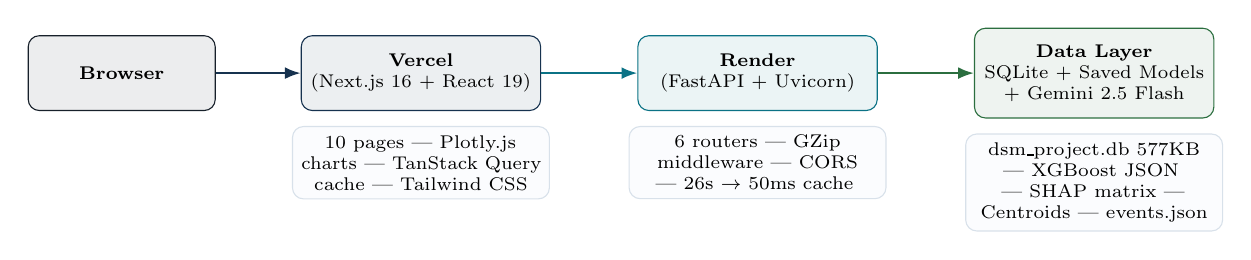
\begin{tikzpicture}[scale=0.95, transform shape, x=1cm,y=1cm,every node/.style={align=center,font=\scriptsize}]
      \node[draw=Ink,fill=Ink!8,rounded corners,minimum width=2.5cm,minimum height=1cm] (browser) at (0,0) {\textbf{Browser}};
      
      \node[draw=Slate,fill=Slate!8,rounded corners,minimum width=3.2cm,minimum height=1cm] (vercel) at (4,0) {\textbf{Vercel}\\(Next.js 16 + React 19)};
      
      \node[draw=Teal,fill=Teal!8,rounded corners,minimum width=3.2cm,minimum height=1cm] (render) at (8.5,0) {\textbf{Render}\\(FastAPI + Uvicorn)};
      
      \node[draw=Forest,fill=Forest!8,rounded corners,minimum width=3.2cm,minimum height=1.2cm] (data) at (13,0) {\textbf{Data Layer}\\SQLite + Saved Models\\+ Gemini 2.5 Flash};
      
      \draw[-{Latex[length=2mm]},thick,Slate] (browser) -- (vercel);
      \draw[-{Latex[length=2mm]},thick,Teal] (vercel) -- (render);
      \draw[-{Latex[length=2mm]},thick,Forest] (render) -- (data);
      
      \node[below=0.2cm of vercel,text width=3.2cm,draw=LineGray,fill=Pale,rounded corners] {10 pages | Plotly.js charts | TanStack Query cache | Tailwind CSS};
      \node[below=0.2cm of render,text width=3.2cm,draw=LineGray,fill=Pale,rounded corners] {6 routers | GZip middleware | CORS | 26s $\rightarrow$ 50ms cache};
      \node[below=0.2cm of data,text width=3.2cm,draw=LineGray,fill=Pale,rounded corners] {dsm\_project.db 577KB | XGBoost JSON | SHAP matrix | Centroids | events.json};
    \end{tikzpicture}
  \end{center}
  \vfill
  {\scriptsize
  \textbf{Dashboard:} dsm-project-phi.vercel.app \hfill
  \textbf{API:} wacmr-api.onrender.com \hfill
  \textbf{Repo:} github.com/AJ112103/DSM\_project}
\end{frame}

% ---------------------------------------------------------------------
% SLIDE 23
% ---------------------------------------------------------------------
\begin{frame}{The Interactive System: Features Showcase}
  \begin{columns}[T,totalwidth=\textwidth]
    \column{0.48\textwidth}
      \card{Slate}{10-Page Dashboard}{
        \begin{itemize}\scriptsize
          \item Comprehensive exploration of WACMR, regimes, forecasts, SHAP drivers, and event context.
          \item Interactive Plotly charts for dynamic filtering.
        \end{itemize}
      }
      \vspace{0.3cm}
      \card{Teal}{Gemini 2.5 Flash Agent}{
        \begin{itemize}\scriptsize
          \item 7 typed tools: run\_sql, run\_counterfactual, get\_shap\_contributions, get\_regime\_stats, search\_columns, query\_schema, get\_event\_context
          \item Loop guard: max 6 iterations
        \end{itemize}
      }
    \column{0.48\textwidth}
      \card{Amber}{Counterfactual Simulator}{
        \begin{itemize}\scriptsize
          \item Slider from $-$200 to +200 bps
          \item Instant WACMR prediction + 90\% confidence interval + SHAP attribution
          \item 26 seconds $\rightarrow$ 50ms via two-layer cache (500$\times$ speedup)
        \end{itemize}
      }
      \vspace{0.3cm}
      \card{Forest}{Blog + Live Report}{
        \begin{itemize}\scriptsize
          \item 11-section technical narrative
          \item Embedded live charts \& scroll-spy TOC
          \item Inline counterfactual widget
          \item Full report with all 12 figures
        \end{itemize}
      }
  \end{columns}
\end{frame}

% ---------------------------------------------------------------------
% SLIDE 24
% ---------------------------------------------------------------------
\begin{frame}{Quality Assurance and Reproducibility}
  \begin{columns}[T,totalwidth=\textwidth]
    \column{0.48\textwidth}
      {\color{Slate}\bfseries Playwright Audit Results}\par
      \vspace{0.1cm}
      {\scriptsize
      \begin{tabularx}{\linewidth}{@{}Yccc@{}}
        \toprule
        \textbf{Page} & \textbf{Desktop ms} & \textbf{Mobile ms} & \textbf{Status} \\
        \midrule
        Dashboard & < 500 & < 600 & Green \\
        Simulator & < 400 & < 500 & Green \\
        Agent & < 800 & < 900 & Green \\
        Report & < 600 & < 700 & Green \\
        \dots & \dots & \dots & \dots \\
        \bottomrule
      \end{tabularx}}
      \vspace{0.1cm}
      \callout[Teal]{\textbf{Summary:} 20 tests total | 0 console errors | 0 network failures | All green}
    \column{0.48\textwidth}
      {\color{Slate}\bfseries Reproducibility Checklist}\par
      \vspace{0.1cm}
      \begin{itemize}\scriptsize
        \item[\checkmark] All Python packages pinned to specific versions
        \item[\checkmark] Pipeline stages idempotent (run twice = same result)
        \item[\checkmark] Random seeds fixed (K-Means: 42, XGBoost: deterministic)
        \item[\checkmark] SQLite database committed to repo
        \item[\checkmark] Saved model artefacts committed (XGBoost JSON, SHAP matrix, centroids)
      \end{itemize}
  \end{columns}
\end{frame}

% ---------------------------------------------------------------------
% SLIDE 25
% ---------------------------------------------------------------------
\begin{frame}{Limitations and Future Work}
  {\color{Slate}\bfseries Honest Constraints and Next Steps}\par
  \vspace{0.2cm}
  {\scriptsize
  \begin{tabularx}{\linewidth}{@{}p{0.45\linewidth}Y@{}}
    \toprule
    \textbf{Limitation} & \textbf{Future Work} \\
    \midrule
    Target substitution (T-Bill yields unavailable $\rightarrow$ switched to WACMR) & Retrain once NDAP publishes T-Bill yields \\
    Two-regime simplicity (K=3 only 0.019 worse) & Try HDBSCAN / hierarchical clustering \\
    17.4\% imputation on 2 columns & Sensitivity analysis without imputed columns \\
    Single one-week horizon only & Multi-horizon models with conformal prediction \\
    Single-target regression & Vector autoregression for joint rate dynamics \\
    No causal identification & Synthetic control for specific policy events \\
    75-event NLP corpus too small for strong signal & FinBERT pipeline over full RBI press release archive ($\sim$5,000 documents) \\
    No event dummies for surprise inter-meeting actions & Add MPC calendar binary dummy \\
    \bottomrule
  \end{tabularx}}
\end{frame}

% ---------------------------------------------------------------------
% SLIDE 26
% ---------------------------------------------------------------------
\begin{frame}{Conclusion: The Headline Numbers}
  \begin{columns}[T,totalwidth=\linewidth]
    \column{0.32\linewidth}\kpi{0.1019 RMSE}{($\sim$10 basis points)}{}
    \column{0.32\linewidth}\kpi[Forest]{70.9\%}{Directional Accuracy}{}
    \column{0.32\linewidth}\kpi[Teal]{0.4238}{Silhouette Score}{}
  \end{columns}
  \vspace{0.4cm}
  \card{Slate}{1. The 2020 structural break is real}{K-Means found it without being told a single date.}
  \vspace{0.1cm}
  \card{Teal}{2. The corridor explains WACMR; equity and forex features do not}{Empirically confirmed, not assumed.}
  \vspace{0.1cm}
  \card{Rose}{3. Calendar pressure is not the forecasting problem}{Genuine policy surprises are.}
  \vfill
  \callout[Amber]{\textbf{Takeaway:} India's overnight call-money rate is corridor-bound, regime-structured, and predictable to $\sim$10 basis points from open public data alone.}
\end{frame}

% ---------------------------------------------------------------------
% SLIDE 27
% ---------------------------------------------------------------------
\begin{frame}[plain]
  \begin{center}
    {\usebeamerfont{title}\color{Slate}Thank You\par}
    \vspace{0.2cm}
    {\usebeamerfont{subtitle}\color{Teal}Questions Welcome\par}
    \vspace{0.6cm}
    
    \begin{columns}[T,totalwidth=\textwidth]
      \column{0.32\textwidth}
        \card{Slate}{Dashboard}{dsm-project-phi.vercel.app}
      \column{0.32\textwidth}
        \card{Teal}{API}{wacmr-api.onrender.com}
      \column{0.32\textwidth}
        \card{Forest}{GitHub}{github.com/AJ112103/DSM\_project}
    \end{columns}
    
    \vspace{0.8cm}
    {\large Aamer Jalan \& Arnav Goyal}\\
    {\small Ashoka University | Data Science and Management}
  \end{center}
  \vfill
  \callout[Slate]{\centering All figures reproducible from committed pipeline stages 1–6}
\end{frame}

\end{document}
